\chapter{Literature review}

\ifpdf
    \graphicspath{{Chapter2_LitReview/Chapter2Figs/PNG/}{Chapter2_LitReview/Chapter2Figs/PDF/}{Chapter2_LitReview/Chapter2Figs/}{Chapter2_LitReview/Chapter2Figs/Classification/}{Chapter2_LitReview/Chapter2Figs/Detection/}{Chapter2_LitReview/Chapter2Figs/Restoration}}
\else
    \graphicspath{{Chapter2_LitReview/Chapter2Figs/EPS/}{Chapter2_LitReview/Chapter2Figs/}}
\fi

The literature review presented in this chapter is split into 3 major sections. Classification, Detection and Restoration. These 3 major areas will generally be dealt with in the order in which they are relevant.

%Not JUST classification. Also some other stuff (needs to be removed)
\section{Classification}\label{sec:LitRev_Classification}
\subsection{Computational Auditory Scene Analysis (CASA)}
The CASA approach to source separation attempts to mimic the Auditory Scene Analyzing (ASA) capabilities of the brain by computational means. \cite{Wang2006} state: ``One may define the CASA problem as the challenge of constructing a machine learning system that achieves human performance in ASA''. In an attempt to make CASA systems more \emph{biologically relevant} many CASA systems limit their scope to either monaural or binaural input signals and hence replicating the ASA problem where only the signal from the two ears are present.

More specifically CASA solutions aim to identify certain auditory object, such as characterizing note objects in terms of harmonicity, correlated modulation, duration of sinusoidal partials and common onset, and arranging these into streams using psycho-acoustic cues \citep{Ellis1996}. Proximity of time-frequency objects within the audio mixture can cause problems for CASA whereas ASA is able to retain a reasonable degree of separation of sources. These shortcomings of CASA have thus been the focus of much research. Examples of this is the integration of evidence derived from multiple grouping principles at several levels of abstraction \citep{Godsmark1999}, matching of timbre features learned on solo excerpts \citep{Kashino1998},\citep{Kinoshita1999},\citep{Eggink2003} (based on a Gaussian Mixture Model (GMM) classifier). More recently the overlap probability of frequency components has been introduced to improve algorithm performance \citep{Sakuraba2003}.

CASA methods still suffer from a few drawbacks though. The brain's own ASA system is able to localize sources in a natural acoustic environment through what is known as the \emph{precedence effect}. In environments where a sound is reflected multiple times before reaching the listener, the brain is able to give \emph{precedence} to early arrival of sounds, such as the direct sound, and hence evaluate the true location of the sound. This precedence rule between grouping cues can be hard to assess \citep{Wang2006}, which is also why current methods are restricted to non-reverberant mixtures \citep{Vincent2006}.

In the recent paper, \cite{Shao2010}, the authors present a CASA system for separating speech signals in the presence of other speech or noise. Their approach proceeds by tracking time-frequency units across time frames in 2 different stages. Firstly they use harmonicity to segregate the voiced portions of individual sources for each time frame using multipitch tracking. Secondly the time-frequency units are grouped across the time frames by utilizing knowledge from the speaker characteristics. The system proposed in \cite{Shao2010} mainly focusses on features such as onset/offset and periodicity which are not specific necessarily specific to the target source or even speech and as such this system works well for a variety of speech separation cases with a variety of noise scenarios.

\subsection{Independent Component Analysis (ICA)}
One of the most widely known and used methods for blind source separation (BSS) is Independent Component Analysis (ICA). ICA proposes to separate a multivariate signals into additive subcomponents supposing the mutual statistical independence of the non-Gaussian source signals. For $M$ observations and $N$ sources it is a requirement for ICA to work that $M\geq N$.
In general ICA can be defined as the linear transformation $\textrm{\textbf{A}}$ of observed data $\textrm{\textbf{x}} = [x_1,\ldots,x_M]$

\begin{equation}\label{eq:ICA1}
    \textrm{\textbf{x}} = \textrm{\textbf{A}}\textrm{\textbf{s}}
\end{equation}

where $\textrm{\textbf{s}}  = [s_1,\ldots,s_N]$ is the separated sources or components \citep{Virtanen2007}.

Traditionally $\textrm{\textbf{A}}$ would then be referred to as the mixing matrix. The source signals $\textrm{\textbf{s}}$ can feasibly be recovered using $\textrm{\textbf{s}} = \textrm{\textbf{A}}^{-1}\textrm{\textbf{x}}$  with $\textrm{\textbf{A}}$ the invertible matrix.  $\textrm{\textbf{A}}^{-1}$ is then called the un-mixing matrix \citep{Smaragdis1998}.

A very popular implementation of the ICA method is the FastICA algorithm as proposed in \cite{Hyvarinen1999}. Often mixture models are modeled as \emph{convolutive} and hence solving for the mixing matrix \textbf{A} in the time-domain will require labor-intensive convolution while some methods propose solutions to the inherent permutation problem for the frequency domain equivalent of the FastICA \citep{Mitianoudis2003}. It has been reported that this approach has also produced good separation results.

A more recent paper \citep{Douglas2007} presents two spatio-temporal extensions to the FastICA method and reports significant improvements over previous methods when applied to multichannel recordings of two- and three-source speech mixtures in a room environment. It was also noted that this proposed method was simple, fast and did not require parameter tuning in order to obtain good separation performance.

\subsubsection{Convolutive mixtures}
Due to extensive filtering imposed upon real world signals by their environment and propagation delays, instantaneous mixtures are rarely encountered. Most real world mixtures tend to be of convolved mixtures \citep{Smaragdis1998}.

Consider again the model from equation~(\ref{eq:ICA1}) but this time consider a mixture $\textrm{\textbf{x}}$ recorded in a real environment where the mixture can be approximated by a convolutive mixture of the source signals in the time domain,

\begin{equation}\label{eq:ICA2}
    \textrm{\textbf{x}}(t) = \textrm{\textbf{A}}(t) \ast\textrm{\textbf{s}}(t).
\end{equation}

Applying the Fourier Transform (FT) yields:
\begin{equation}\label{eq:ICA3}
   \hat{ \textrm{\textbf{x}}}(\omega) = \hat{\textrm{\textbf{A}}}(\omega)\hat{\textrm{\textbf{s}}}(\omega),
\end{equation}
where $\hat{ \textrm{\textbf{x}}}(\omega), \hat{\textrm{\textbf{A}}}(\omega)$ and $\hat{\textrm{\textbf{s}}}(\omega)$ are the FT of $\textrm{\textbf{x}}(\omega), \textrm{\textbf{A}}(\omega)$ and $\textrm{\textbf{s}}(\omega)$ respectively \citep{Ikeda1999}.

It is noted that if $\textrm{\textbf{A}}$ in equation~(\ref{eq:ICA1}) is seen as a matrix of FIR filters instead of scalars, the resulting multiplication will be equivalent to convolution and the notation will be consistent. This notation is called FIR algebra notation \citep{Lambert1996}.

This time-frequency approach to ICA has been proposed by a variety of authors \citep{Lee1998},\citep{Ikeda1999},\citep{Smaragdis1998} and specifically \cite{Ikeda1999} has been successful in dealing with the inherent arbitrary scaling and permutation problems of the ICA approach applied in a frequency domain context \citep{Zhang2007}.

The recent paper \cite{Zhang2007} attempts to avoid the whitening of outputs which plagues conventional implementations of ICA for convolutive mixtures by enforcing pairwise independence rather than mutual independence. This approach is based on the findings that for blind separation the two are generally equivalent.
%better ending here?

\subsection{Independent Subspace Analysis (ISA)}
Independent Subspace Analysis (ISA) is based on ICA but relaxes the constraints $M\geq N$ and the statistical independence of source signals. In practice ISA is a generalization of ICA in the sense that instead of requiring statistical independence between components ISA requires statistical independence between groups of components. ISA can also been described as multidimensional independent component analysis and hence the independent components are required to be of the same dimension $k$. In the case where $k = 1$, ISA is equivalent to ICA \citep{Theis2006}. Despite this relaxing of restrictions of the ICA approach implementations of ISA has still been restricted by fixed group sizes or semi-parametric models. An even more general approach has been proposed which introduces the concept of irreducible independent components and give an identifiability result for this general, parameter-free model together with an arbitrary subspace size algorithm \citep{Theis2006}.

A previous study managed to implement ISA models for audio source separation and introduced the \emph{ixegram} as a measure space for grouping independent basis components \citep{Casey2000}. The separation and grouping results from this experiment suggest that the technique can perform separation of source signals without parametric model fitting or prior knowledge of the composition of input data.

\subsection{Non-Negative Matrix Factorisation (NMF)}
Since the concept of Non-Negative Matrix Factorization (NMF) was introduced independently by \cite{Paatero1997} and \cite{Lee1999} the method has gained some popularity within the field of polyphonic transcription and the source separation field \citep{Smaragdis2003},\citep{Smaragdis2004}. NMF was originally proposed as an alternative to $k$-means clustering and principal component analysis (PCA) for data analysis and compression.
The original formulation of NMF starts with a non-negative $M\times N$ matrix $\textrm{\textbf{V}} \in \mathbb{R}^{\geq 0,M\times N}$ where the goal is to approximate $\textrm{\textbf{V}}$ as a product of two non-negative matrices so that

\begin{equation}\label{eq:nmf1}
    \textrm{\textbf{V}} \approx \textrm{\textbf{W}}\textrm{\textbf{H}}
\end{equation}
where $\textrm{\textbf{W}} \in \mathbb{R}^{\geq 0,M\times R}$, $\textrm{\textbf{H}} \in \mathbb{R}^{\geq 0,R\times N}$ and $R \leq M$ such that the error of reconstruction is minimized \citep{Smaragdis2004}.

Good results have generally been reported for extraction of percussive sounds in mono recordings, but for low intensity sounds the algorithms generally perform worse and suffer from distortion and lost information inherent in the mixing and analysis process \citep{Smaragdis2004}. Other results have shown NMF to consistently obtain better separation results than ISA and ICA \citep{Virtanen2007}.

\subsection{Hierarchical Bayesian Models}
The task in Bayesian source separation is to infer $N$ source signals $s_{k,n} \equiv \textrm{\textbf{s}}$ given $M$ observed signals $x_{k,m} \equiv \textrm{\textbf{x}}$, where $n=[1,\ldots,N]$ and $m=[1,\ldots,M]$. Here $k=[1,\ldots,K]$ is an index which may correspond to time or to expansion coefficient of the sources in a linear transform domain. A Hierarchical Bayesian Model for the inference of the source signals can hence be formulated as

\begin{equation}\label{eq:hbm1}
    p(\textrm{\textbf{s}}|\textrm{\textbf{x}}) = \frac{1}{Z_x}\int p(\textrm{\textbf{x}}|\textrm{\textbf{s}},\Theta_m)p(\textrm{\textbf{s}}|\Theta_p)p(\Theta_p)p(\Theta_m)d\Theta_m d\Theta_p.
\end{equation}

Here the conditional distribution is characterized by the conditional distribution $p(\textrm{\textbf{x}}|\textrm{\textbf{s}},\Theta_m)$, where $\Theta_m$ denotes the collection of mixing parameters such as the mixing matrix, observation noise and variance, etc. and the prior term $p(\textrm{\textbf{s}}|\Theta_p)$ describes the sources via their own prior parameters $\Theta_p$ \citep{Cemgil2007}.

It is worth noting that there is a considerable computational cost associated with a full Bayesian inference, via MCMC or Variational Bayes for Bayesian source separation (VB). Good results were reported in a study attempting Bayesian source separation using an MCMC approach to inference \citep{Fevotte2006}. Also, the authors of this study point out the computational burden of the MCMC approach compared to the alternative Expectation Maximisation (EM) approach. It was although also noticed that the EM approach was far more sensitive to mixing matrix initialization and hence less robust. The Gibbs sampler described in this paper was implemented as part of the review of this paper. Although the implementation was problematic due to the inherent indeterminacy on gain, the approach provided good results to noisy linear mixtures of sources.

The recent paper \cite{Cemgil2007} describes a hybrid approach where a general linear instantaneous model, which might be noisy and underdetermined, is tackled using a Student $t$ distribution to model the source prior. Both the Gibbs sampler and VB method were studied as a method for inference. Both these methods are algorithmically similar but by employing a hybrid method the authors managed to combine the speed of the variational approach with the robustness of the Gibbs sampler \citep{Cemgil2007}.

\subsection{Principal Component Analysis (PCA)}
The central idea of PCA is to reduce the number of dimensions of a set of data consisting of possibly correlated variables to a smaller number of uncorrelated variables. This operation is achieved by transforming to a set of uncorrelated variables, principal components (PCs), which are ordered so the first PC retain most of the variability and each succeeding component accounts for as much of the remaining variability as possible.

Take $\textrm{\textbf{x}}$ to be a vector of $p$ random variables where the variance of the variables and the correlation or covariance between them are of interest. The approach taken by PCA is to look for a few ($<<p$) derived variables which preserves most of the information given by these variances and covariances or correlations. The initial step is to look for a linear function $\boldsymbol\alpha_1^T \textrm{\textbf{x}}$ of $\textrm{\textbf{x}}$ which maximizes the variance, where $\boldsymbol\alpha_1^T =  [\alpha_{1{}1},\alpha_{1{}2},\ldots,\alpha_{1{}p}]$ so that:

\begin{equation}\label{eq:PCAdef}
\boldsymbol\alpha_1^T \textrm{\textbf{x}}= \alpha_{1{}1}x_1 +\alpha_{1{}1} x_2 + \ldots \alpha_{1{}p} x_p = \sum^p_{j=1}\alpha_{1{}j}x_j,
\end{equation}

is the first PC where ${}^T$ denotes a transposed matrix.
Now, find the linear function $\boldsymbol\alpha_2^T \textrm{\textbf{x}}$ of $\textrm{\textbf{x}}$ uncorrelated with $\boldsymbol\alpha_1^T \textrm{\textbf{x}}$ which again maximizes the variance, and so on, so that the $k$th PC $\boldsymbol\alpha_k^T \textrm{\textbf{x}}$ maximizes the variances while being uncorrelated to $\boldsymbol\alpha_1^T \textrm{\textbf{x}}, \boldsymbol\alpha_2^T \textrm{\textbf{x}}, \ldots, \boldsymbol\alpha_{k-1}^T \textrm{\textbf{x}}$. For a reduction of dimensionality it is hoped that most of the variability of $\textrm{\textbf{x}}$ is accounted for by $q$ PCs where $q<<p$ \citep[chap. 1]{Jolliffe1986}.

A more common transform into uncorrelated basis functions is the Discrete Fourier Transform (DFT) or FT which decomposes a signal into a set of uncorrelated or orthogonal (in the statistical sense) complex exponentials of the form $e^{i\omega t}$. The transform described above can therefore be seen as a generalization of the DFT for random processes, where the decomposed uncorrelated basis functions are real random signals rather than complex exponentials \citep[chap. 4.6]{Therrien1992}.

\subsection{Simple PCA Examples}

Figure~\ref{fig:30observations} gives a plot of 30 observations of two highly correlated (non zero mean) variables $x_1$ and $x_2$. It is seen that although there are considerable variation in the two variables, it is also noticed that there is more variation in the direction $x_2$.
\begin{figure}[!]
  \begin{center}
    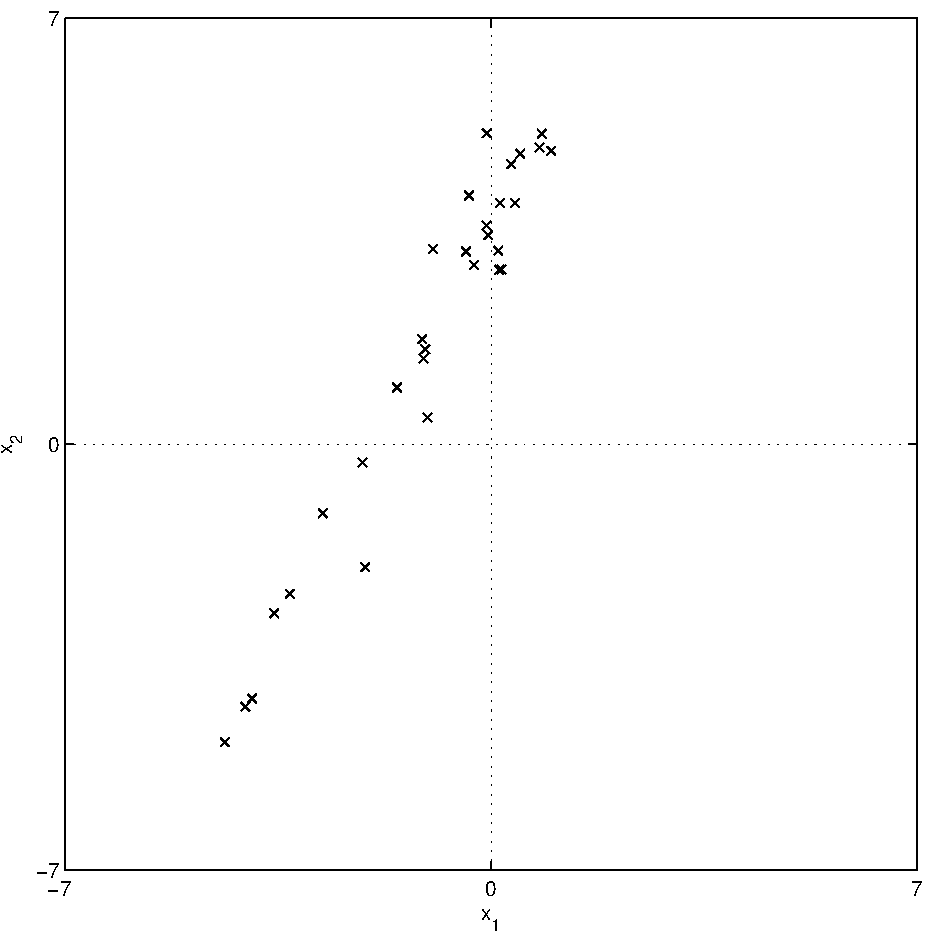
\includegraphics[width=260px]{30observations.pdf}
    \caption{Plot of 30 observations of variables $x_1$ and $x_2$.}\label{fig:30observations}
  \end{center}
\end{figure}

It is also seen in Figure~\ref{fig:30observations} that neither of the two variables are zero mean. To apply PCA the mean of both variables must be subtracted. Figure~\ref{fig:30observationsBar} shows the two variables with their means subtracted.
\begin{figure}[!]
  \begin{center}
    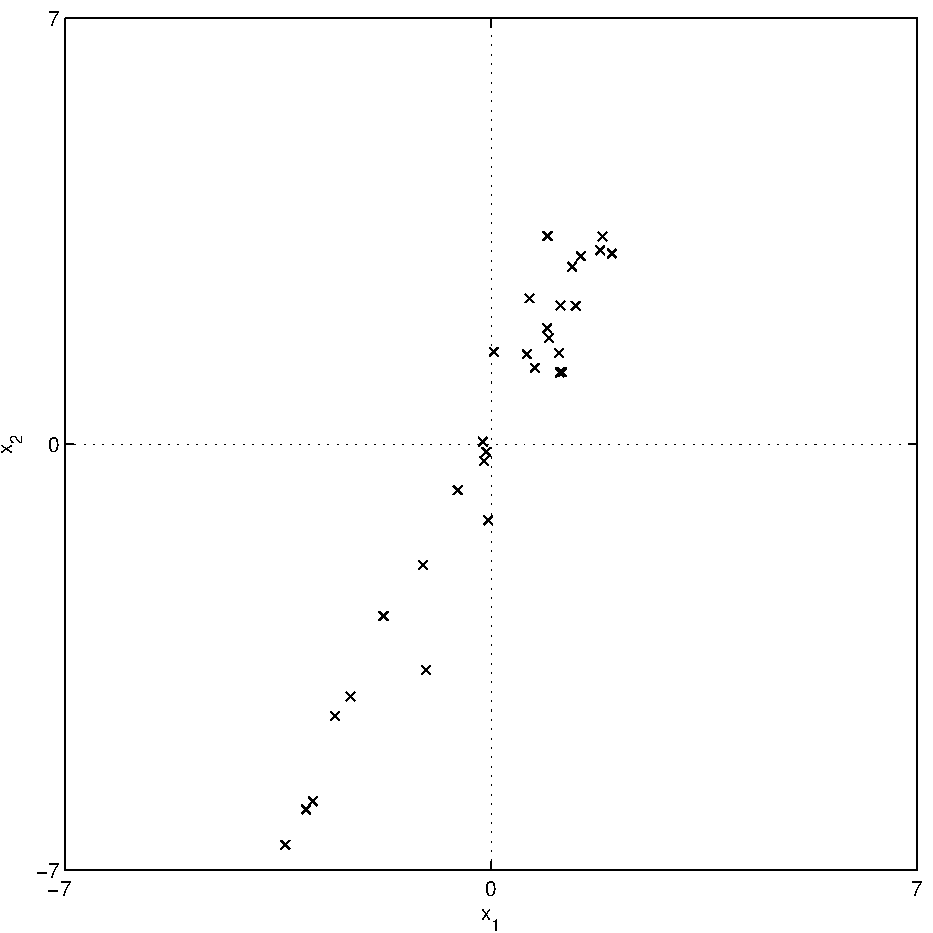
\includegraphics[width=260px]{30observationsBar.pdf}
    \caption{Plot of 30 observations of variables $x_1$ and $x_2$ with means subtracted.}\label{fig:30observationsBar}
  \end{center}
\end{figure}

Since the process of PCA is closely related to the diagonalization of the correlation matrix \citep[p. 174]{Therrien1992}, a helpful interpretation of the PCA is the attempt to ``rotate'' the axes of Figure~\ref{fig:30observationsBar} to collect as much variability as possible in one dimension, rather than having it spread over 2 dimensions. The correlation matrix (correlation coefficients) for the two variables $x_1$ and $x_2$ is,

\begin{equation}\label{eq:corrcoef}
\textrm{Correlation matrix} = \textrm{corr}(x,y)= \left(
    \begin{array}{cc}
        1   & 0.97 \\
        0.97& 1    \\
    \end{array}\right),
\end{equation}
where the correlated nature of the two variables is clearly seen by the almost unitary off-diagonal terms. Since the covariance matrix $\boldsymbol\Sigma$ is square it is possible to look at the eigenvalues and eigenvectors of it, which are,

\begin{eqnarray}\label{eq:eigValues}
\textrm{Eigenvalues} &=& \boldsymbol\lambda = \left(
    \begin{array}{c}
        \lambda_1 \\
        \lambda_2 \\
    \end{array}\right) = \left(
    \begin{array}{c}
        11.85 \\
        0.107 \\
    \end{array}\right)\\\label{eq:eigenVectors}
    \textrm{Eigenvectors} &=& \boldsymbol\alpha = \left( \boldsymbol\alpha_1 \quad \boldsymbol\alpha_2\right) =\left(
    \begin{array}{cc}
         0.451 & -0.892  \\
         0.892 & 0.451   \\
    \end{array}\right).
\end{eqnarray}

The eigenvectors from equation~(\ref{eq:eigenVectors}) have been plotted on top of the data in Figure~\ref{fig:30observationsBarEig}. These eigenvectors reveal information about patterns in the data, and as expected a clear correlation is found by the eigenvector $\boldsymbol\alpha_1$ between the variables $x_1$ and $x_2$. The second eigenvector $\boldsymbol\alpha_2$ gives the other, less important, pattern in the data.

\begin{figure}[!]
  \begin{center}
    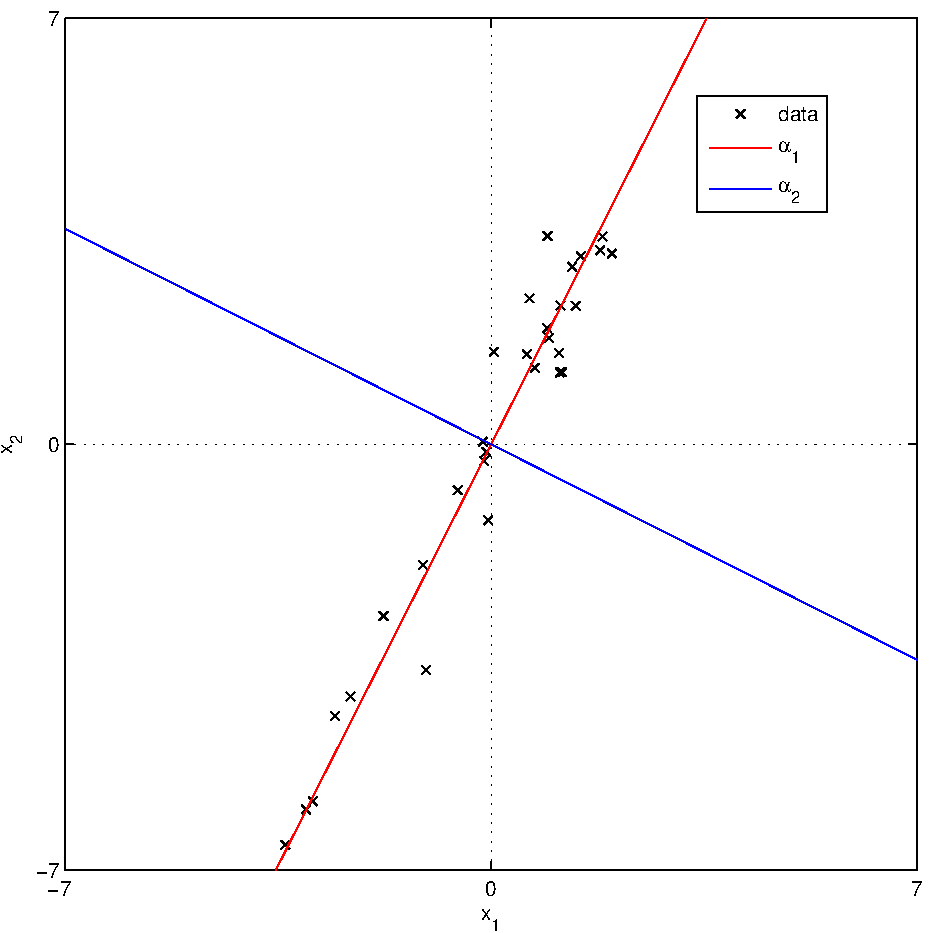
\includegraphics[width=260px]{30observationsBarEig.pdf}
    \caption{Plot of 30 observations of variables $x_1$ and $x_2$ with means subtracted, and eigenvectors of covariance matrix $\boldsymbol\Sigma$ plotted on top of the data. $\boldsymbol\alpha_k$ refers to the $k$th eigenvector.}\label{fig:30observationsBarEig}
  \end{center}
\end{figure}

The eigenvector with the highest corresponding eigenvalue is the PC. Ordering the eigenvectors in terms of descending eigenvalue gives the components in order of significance. It turns out that, for $k \in \{1, 2, \ldots, p\}$ the $k$th PC is given by $z_k = \boldsymbol\alpha_k^T\textrm{\textbf{x}}$, where $\textrm{\textbf{x}} = [x_1,x_2,\ldots, x_p]^T$ and where $\boldsymbol\alpha_k$ corresponds to the eigenvector with the $k$th largest eigenvalue \citep[p. 2-3]{Jolliffe1986}. For a complete transformation of the data use the expression $\textrm{\textbf{z}} = \hat{\boldsymbol\alpha}^T\textrm{\textbf{x}}$ where $\hat{\boldsymbol\alpha}$ is the feature vector containing the number of eigenvectors desired $q$, so $\hat{\boldsymbol\alpha} = [\boldsymbol\alpha_1,\boldsymbol\alpha_2,\ldots,\boldsymbol\alpha_q]$. Figure~\ref{fig:30observationsBarEig} shows the transformed data in terms of the transformed variables $z_1$ and $z_2$.

\begin{figure}[!]
  \begin{center}
    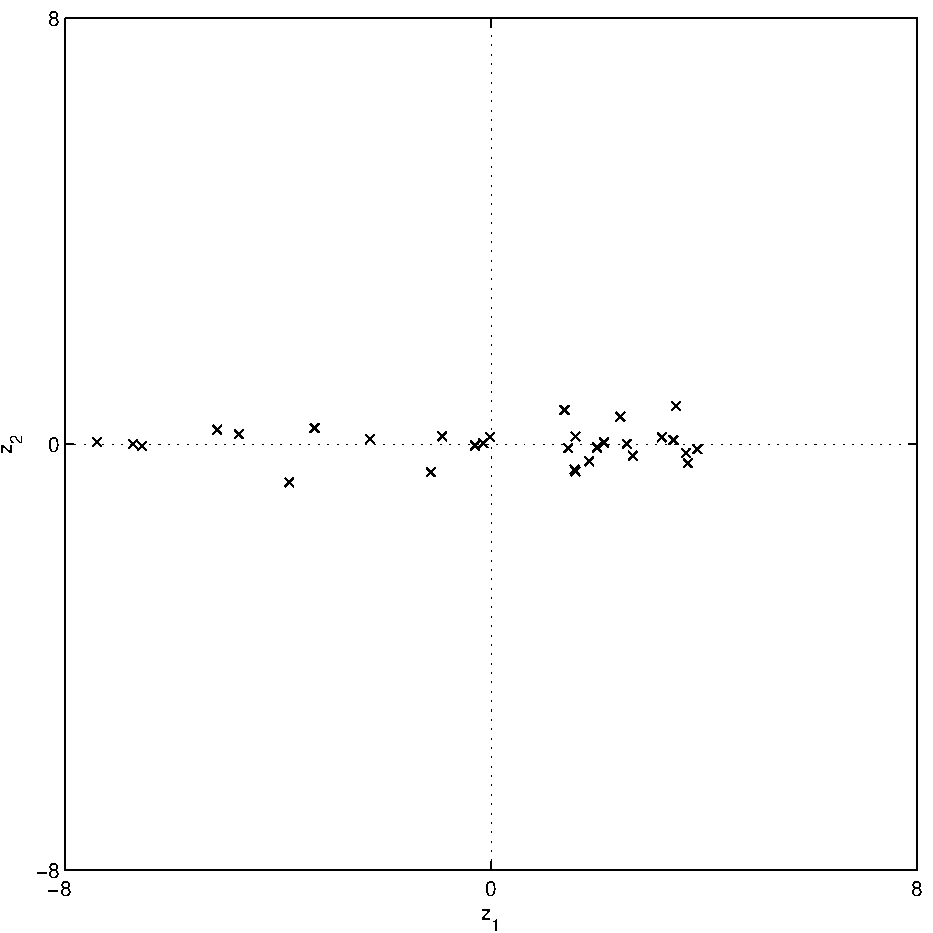
\includegraphics[width=260px]{30observationsBarTrans.pdf}
    \caption{Plot of 30 observations of variables $x_1$ and $x_2$ transformed into $z_1$ and $z_2$. Almost all the information or variability is now in $z_1$.}\label{fig:30observationsBarTrans}
  \end{center}
\end{figure}

It is noticed that this transform, who's results are displayed in Figure~\ref{fig:30observationsBarEig}, do not actually reduce the dimensionality of the data since $q=p$ and hence all information is preserved. By making $q<p$ the dimensionality is reduced and less significant data is discarded. Since it is noticed from equation~(\ref{eq:eigValues}) that $\lambda_1$ is much larger than $\lambda_2$, and hence $\boldsymbol\alpha_1$ is a far more significant component in the data than $\boldsymbol\alpha_2$, one could feasibly define the feature vector as $\hat{\boldsymbol\alpha} = \boldsymbol\alpha_1$. Figure~\ref{fig:30observationsFinal} shows the result of a transformation of the 30 observations for this scenario where $q=1$. The data has been transformed back into $x_1$ and $x_2$ and the original means of the data has been reapplied.

\begin{figure}[!]
  \begin{center}
    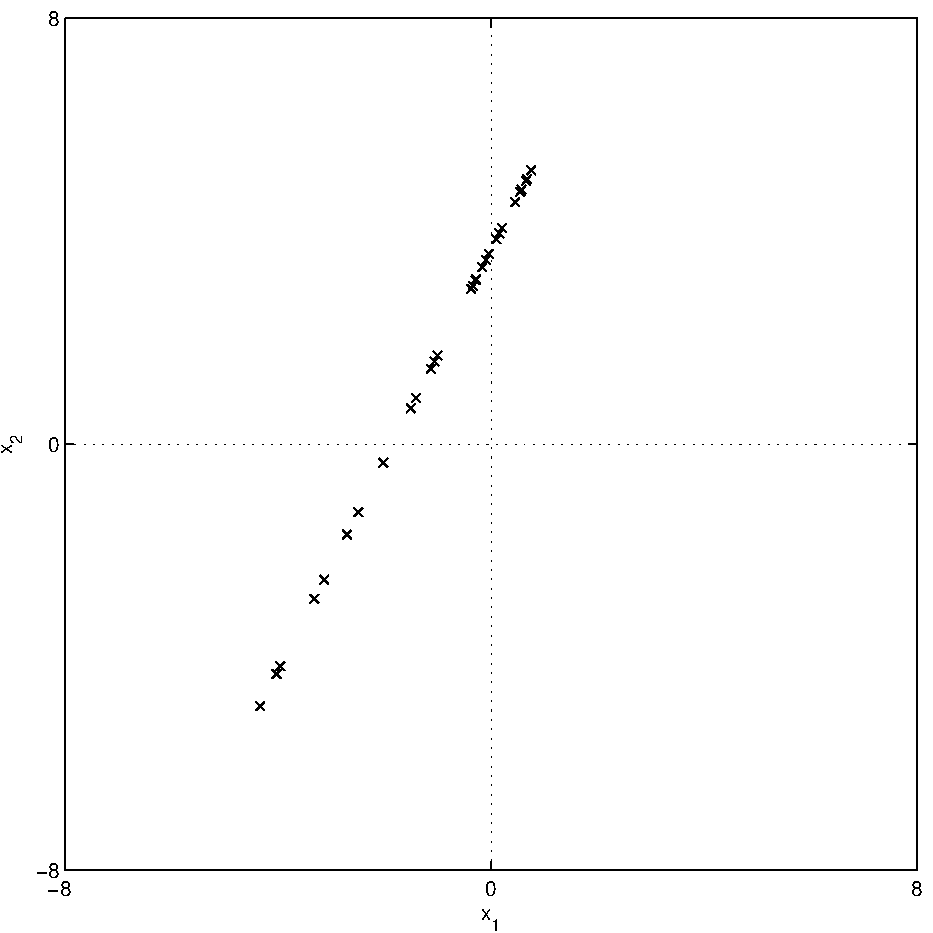
\includegraphics[width=270px]{30observationsFinal.pdf}
    \caption{Plot of 30 observations of variables $x_1$ and $x_2$ transformed from only $z_1$ with original means added back in.}\label{fig:30observationsFinal}
  \end{center}
\end{figure}

It is clearly seen how the data resembles that of Figure~\ref{fig:30observations} although some of the variability has been lost in the dimensional reduction.

\subsubsection{Eigenfaces}
A popular application of PCA is the so called \emph{eigenfaces}. \emph{Eigenfaces} are essentially eigenvectors derived from the covariance matrix of a high dimensional vector space or ensemble of individual pictures. The idea of \emph{eigenpictures} was originally developed by \cite{Sirovich1987} were the authors repeatedly draw parallels between how humans recognize facial features and their own computational method. Although the \emph{eigenpictures} were not formerly used for facial recognition until \cite{Turk1991}, where the term \emph{eigenfaces} was first coined, \cite{Sirovich1987} hypothesises that perhaps humans compartmentalize faces and treat different features individually. This assertion is rooted first in the observation that humans are able to store and recognize enormous numbers of faces and secondly, that since recognition is apparently instantaneous it is conceivable that we do it by some efficient method, possibly similar to low dimensional methods. It is for example noted that ``(...) fewer than 100 \emph{eigenpictures} are necessary to fit a picture.'' and ``fewer than 100 dimensions are needed to provide likeness.''.

The method used in \cite{Sirovich1987} uses photographs of 115 male undergraduates faces. These pictures were then digitized to a 128 by 128 pixel image and manually aligned. Figure~\ref{fig:Sirovich1987-3} shows a figure of 3 cropped images. The left image is the average face based on the ensemble, the middle is a sample face and right image that sample faces departure from the ensemble average or the samples \emph{caricature}. All pictures presented in this section are lifted from the original paper \cite{Sirovich1987} where none of the pictures have been filtered to eliminate the high frequencies produced by digitization.

\begin{figure}[!]
  \begin{center}
    \includegraphics[width=410px]{Sirovich1987-3.pdf}
    \caption{Cropped faces: left, the average; middle, a sample face; right, its caricature.}\label{fig:Sirovich1987-3}
  \end{center}
\end{figure}

The covariance matrix of the aligned ensemble is now calculated and all the \emph{eigenpictures} determined. Figure~\ref{fig:Sirovich1987-4} shows the first 8 of these \emph{eigenpictures} going from the top left frame, moving right and ending on the bottom right frame with the 8th \emph{eigenpicture}.

\begin{figure}[!]
  \begin{center}
    \includegraphics[width=270px]{Sirovich1987-4.pdf}
    \caption{First 8 \emph{eigenpictures} starting at upper left, moving to the right, and ending at lower right.}\label{fig:Sirovich1987-4}
  \end{center}
\end{figure}

Figure~\ref{fig:Sirovich1987-5} shows the approximate reproduction of the sample face from Figure~\ref{fig:Sirovich1987-3} reproduced using 10, 20, 30 and 40 components.

\begin{figure}[!]
  \begin{center}
    \includegraphics[width=270px]{Sirovich1987-5.pdf}
    \caption{Approximation of the original picture (middle picture of Figure~\ref{fig:Sirovich1987-3}) using 10, 20, 30 and 40 \emph{eigenpictures}.}\label{fig:Sirovich1987-5}
  \end{center}
\end{figure}



\subsubsection{In the literature}
As mentioned previously, one of the main applications of PCA is dimensionality reduction which has rendered it useful in a variety of compression applications. Within the image compression community \citep{Vasilescu2003} the focus on PCs has been useful in dimensionality reduction, and more specifically it has been widely applied as a way of representing animations of 3D geometric shapes. \cite{Alexa2000} presented an ``easy and adaptive lossy compression'' algorithm which provided compression of animation sequences with a factor of 1:100 accepting loss in animation accuracy. Another approach to animation compression is presented in \cite{Karni2004} where PCA is combined with Linear Prediction Coding (LPC) to individually focus on spatial and the resulting temporal components respectively.

Although PCA is optimal in approximating the input data in the mean-squared error sense, the representation that it provides is often not the most meaningful in terms of real world data and in terms of describing the fundamental properties of the data. Since the PCA describes the data in an orthonormal basis, purely in order of the second-order statistics (covariance) of the input data \citep{Oja1995}, which in effect means that PCA is networks are only able to realize linear input-output mappings \citep{Karhunen1995}. In the field of neural networks there has been an interest in the development of nonlinear PCA methods that take higher-order statistics into account.

Although not specifically a PCA approach, \cite{Honkela2005} presents an approach to general nonlinear generative model for non-linear factor analysis which can form the basis for many non-linear implementations of latent variable models such as a non-linear generalization of PCA or even ICA. This general model is based on the variational Bayesian framework, which forms a solid foundation for non-linear modeling \citep{Honkela2005}. This model can be implemented into a linear ICA framework for nonlinear BSS, and especially \cite{Valpola2003} found that the variational Bayesian method provided ``useful'' results for difficult nonlinear problems. \citep{Lappalainen2000} introduced nonlinear counterparts of PCA and ICA where the generative mapping from sources to data is not restricted to being linear. Here this mapping is modeled by a multi-layer perceptron (MLP) network and the distributions of source signals are modeled by Gaussians. The general form of the models discussed in this paper are of the form:

\begin{equation}\label{eq:nonlinear}
\textbf{x}(t) = f\left(\textbf{s}(t)\right) + \textbf{n}\left(t\right),
\end{equation}

where $\textbf{x}(t)$ are the observations at time $t$, $\text{s}(t)$ are the sources, $\textbf{n}(t)$ the noise and $f()$ the function which maps the sources to the observation space. In \cite{Lappalainen2000} the authors compare their approach favorably to previously suggested models for representing data with nonlinear coordinate systems, and they especially focus on their methods applicability in high dimensional applications.

%*** Check for more recent papers by MacKay ***

\subsection{Probabilistic PCA (PPCA)}
One of the notable features of the above derived definition of the PCA is the lack of a probabilistic model for the observed data. \cite{Tipping1999} proposes a latent variable model for determining the principal axis of observed data which is closely related to factor analysis. This model utilizes a Maximum Likelihood (ML) estimator to estimate the parameters of the latent variable model. This model is commonly known as a factor analysis model where the relationship is linear:

\begin{equation}\label{eq:facAn}
\textrm{\textbf{t}} = \textrm{\textbf{W}}\textrm{\textbf{x}} + \boldsymbol\mu + \boldsymbol\epsilon,
\end{equation}

in which the $d$-dimensional observations vector \textbf{t} is related to a corresponding $q$-dimensional vector of latent (or unobserved) variables \textbf{x}. The $d \times q$ matrix \textbf{W} relates the two sets of variables, $\boldsymbol\epsilon$ is a zero-mean Gaussian noise process and the parameter $\boldsymbol\mu$ allows for model to have a non-zero mean. By defining $\textrm{\textbf{x}} \sim \mathcal{N}_\textrm{x}(\boldsymbol0,\textrm{\textbf{I}})$ and $\boldsymbol\epsilon \stackrel{i.i.d.}{\sim} \mathcal{N}_\epsilon(\boldsymbol0,\boldsymbol\Psi)$, equation~(\ref{eq:facAn}) induces a Gaussian distribution for the observations $\textrm{\textbf{t}} \sim \mathcal{N}(\boldsymbol\mu,\textrm{\textbf{W}}\textrm{\textbf{W}}^T + \boldsymbol\Psi)$. The parameters of this model can then be obtained through an iterative process using ML \citep{Tipping1999}.

\cite{Lawrence2005} presents an extended PPCA model based on the work of \cite{Tipping1999} termed Dual Probabilistic PCA (DPPCA). The DPPCA method can, through Gaussian processes, nonlinearize the linear mappings from the embedded space and hence provide new probabilistic approach to visualizing and modeling of high dimensional data.
\section{Detection}\label{sec:LitRev_Detection}

Any restoration of transient noise events presupposes complete knowledge of the position of the corruption. In practice this information is unknown \emph{a priori} and some a detection procedure must be employed to ascertain the timing of the corruptions. As noted in this section, a large number of different approaches to transient noise detection has been studied, and since there are as many types of transient noise as there are data that can be corrupted by it, the  detection methods range from simple \emph{ad hoc} filtering approaches to more complicated model based approaches.

In a reconstruction algorithm it is important to focus our attention on audible corruptions. The audibility of a corruption is not only a function of its amplitude or the energy that it represents, but also the context in which is sits. Physcoacoustically some corruptions may be rendered inaudible through masking effects such as the precedence effect, and hence any restoration effort is wasted or potentially damaging.\todo{Add citation for (An Introduction to the Psychology of Hearing)}

The simplest impulse detection algorithms exploit the relatively sparse nature of many audio, and in particular speech, signals above 9000 Hz in relation to impulsive noise which often exhibits a much smoother and wider frequency characteristics \cite{Subramanya2007}. In \cite{Kasparis1993}\cite{US6795559} the authors preprocess their signals using a High Pass filter to target to the impulsive noise.

\subsubsection{Median filter methods}
A classic impulse noise detection (and restoration) scheme has involved a median filter\cite{Tukey1974}\cite{Lee1985}\cite{Heinonen1985}\cite{Heinonen1987}\cite{Maekivirta1991}\cite{Kasparis1993}.
%explain median filtering
Median filtering for signal smoothing, first published in \cite{Tukey1974}, has, according to \cite{Brillinger2002}, some important characteristics in that they reduce ``spiky'' noise while preserving jump discontinuities (edges). In \cite{Lee1985} it is noted that the media filter has limited effect on non-impulsive noise and the authors propose a method for augmenting the median filter with a linear filter for added smoothing. This augmentation of the nonlinear media filter approach with a linear filtering approach has become a popular variation of median filtering process for impulsive noise detection and reduction spawning a variety of implementations \cite{Lee1985}\cite{Heinonen1985}\cite{Nieminen1987}\cite{Kasparis1993}\cite{Loveridge1995}. In \cite{Kauppinen2002} it was also noted that the impulse detection algorithm that performed best was the median filter preprocessed by a linear filter. In recent years median based algorithms such as weighted median (WM) filters \cite{Yin1996}\cite{Wang2010} and switching median filters \cite{Abreu1996}\cite{Chen2000}\cite{Chen2001}\cite{Lin2007} have seen a fair bit of attention although the focus of the implementations have almost exclusively been focused on image data.

The authors of \cite{Chandra1998} employ the SD-ROM (Signal Dependent Rank Order Mean) algorithm, similar to the media filter methods, to evaluate the likelihood of each sample being corrupted based on the neighbouring samples. While this algorithm has shown great results in the removal of impulse noise in images \cite{Abreu1996} in \cite{Chandra1998} the method performs best for short, although frequent, noise pulses of the order of a single or a few samples.

Since transient noise events often exhibit a sudden fast change in the signal, one way to detect the onset of a noise event is to detect abrupt nonstationary changes in the dynamics of time series. In \cite{Fancourt2000} the authors employ neural network predictors for this task, while \cite{Kauppinen2002} proposes an iterative discrete derivative method. In \cite{Kauppinen2002} the linear predictor and median hybrid method outperformed the derivative approach and the method described in \cite{Fancourt2000} was never tested on real data but the requirement for training and the inherent detection deadzone does reduce the method's general applicability.

\subsubsection{Autoregressive (AR) methods}
While autoregressive (AR) methods have been used in other fields for detection and restoration of transient noise events \cite{Arakawa1986} these methods were generally pioneered in the field of audio processing in \cite{Vaseghi1988thesis}\cite{Vaseghi1988}\cite{Vaseghi1990}. AR methods are today the basis for many impulse detection algorithms in audio applications\cite{Karjalainen1997}\cite{Esquef2000}\cite{Haermae2000}\cite{Esquef2002}\cite{Kauppinen2002}\cite{Wolfe2005}\cite{Subramanya2007}. The AR method proceeds by considering a sub-frame of the audio data $x_t$ for $ t = \{ 1, \ldots, N \}$. Assuming the data is drawn from a short-term stationary AR process:

\begin{equation}\label{eq:ARmodel}
x_t = \sum_{i=1}^P a_i x_{n-i} + e_t,
\end{equation}

where $e_t$ is the prediction error (or excitation signal) and $\mathbf{a} = \{a_1,\ldots,a_P\}$ is the AR coefficients of order $P$. The transient nature of the impulsive noise pulses will most likely lead to very large prediction errors if an attempt is made to predict its values with previous values of $x_t$. It follows that if an inverse AR filter is applied to an AR signal segment corrupted with transient noise events $y_t$, the prediction error $e_t = y_t - \sum_{i=1}^P a_i y_{n-i}$ is expected to be large when noise events are present while remaining low at other times\cite{Godsill1998book}.

In \cite{Vaseghi1990} the authors find that linear prediction systems, or AR process, are ``adequate for modelling of speech signals whereas they can not model impulsive disturbances.''. This realisation is used to separate out the residual of the LPC model effectively leaving the excitation noise in addition to the transient noise events, similarly to the pre-processing step of the favored approach in \cite{Kauppinen2002}. Since the transient noise pulses are transformed to a scaled version of the impulse response of the inverse LPC filter, and since experimental results conducted by \cite{Vaseghi1990} shows the amplitude of the excitation signal is in the order of $10^{-1}$ to $10^{-4}$ the detection task is greatly simplified. The authors of \cite{Godsill1998} note that the disadvantages with the approach outlined in \cite{Vaseghi1990} is the inability to detect small impulses in the presence of much larger disturbances as well as the introduction of distortion for certain signals. In \cite{Godsill1998} the impulse detection problem is put in a Bayesian framework and extended to non-Gaussian noise pulses.

An adaptation to the basic AR detection method in \cite{Vaseghi1988} uses a matched filter approach to detect transient noise events. The matched filter approach proceeds by considering the transient noise event as the signal and the AR data as the coloured additive noise. \todo{more on matched filter approach. Possibly also some theory}
An inherent problem with the matched filter is its dependence on training. Other methods in the literature model impulsive noise as non-Gaussian heavy-tailed distributions whereof the $\alpha$-stable distribution is particularly popular \cite{Tsihrintzis1997}\cite{Coates2002}. According to \cite{Nikias1995} $\alpha$-stable distributions are good for modeling many types of impulsive noise (including atmospheric and underwater acoustic noise). While the sub-Gaussians methods in \cite{Tsihrintzis1997}\cite{Coates2002} appear to perform well on certain kinds of impulsive noise it is questionable whether they could perform in a real time application with high impulse variability and high sample rates.

Figure~\ref{fig:LitRev_DetectCompare} and~\ref{fig:LitRev_DetectCompare2} compares the output of 4 basic detections schemes discussed up until now. The data presented in Figure~\ref{fig:LitRev_DetectCompare}(a) and Figure~\ref{fig:LitRev_DetectCompare2}(a) is speech data corrupted with keyboard tapping noise sampled at 44.1 kHz. Each primary tapping impulse has been marked as ``Ground Truth'' although secondary impulses can also be seen. Comparing the matched filter (b) and AR prediction error (c) methods in Figures~\ref{fig:LitRev_DetectCompare} and~\ref{fig:LitRev_DetectCompare2} is is noted that the matched filter produces a more smeared response while, in some cases, picking out more subtle impulses\cite{Godsill1998book}, e.g. 3rd marked impulse in Figure~\ref{fig:LitRev_DetectCompare}.
\todo{Compare (d) and (e) in figures... but mention that they are similarly performing for this data.}

\begin{figure}[!] %LitRev_DetectCompare
\centering
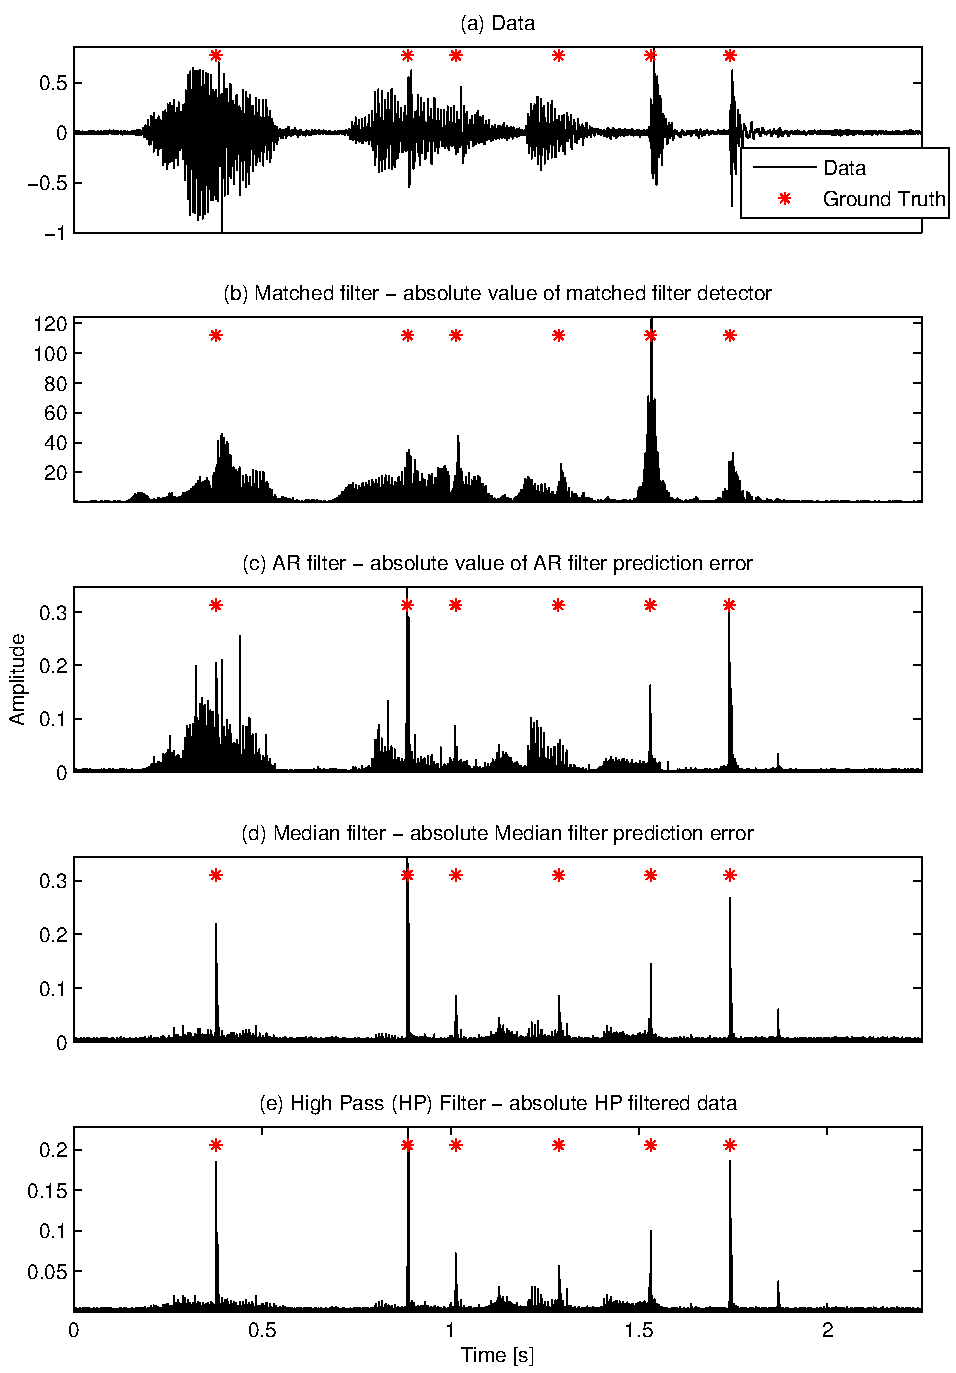
\includegraphics[width=130mm]{LitRev_DetectCompare.pdf}
\caption{Impulse detection comparison, (a) Speech data with 6 primary keystroke impulses sampled at 44.1 kHz, (b) absolute value matched filter detector output, (c) absolute value of AR filter prediction error output, (d) absolute value of median filter prediction error, and (e) absolute value of high pass filtered data with crossover frequency 9.6 kHz.}
\label{fig:LitRev_DetectCompare}
\end{figure}

\begin{figure}[!] %LitRev_DetectCompare2
\centering
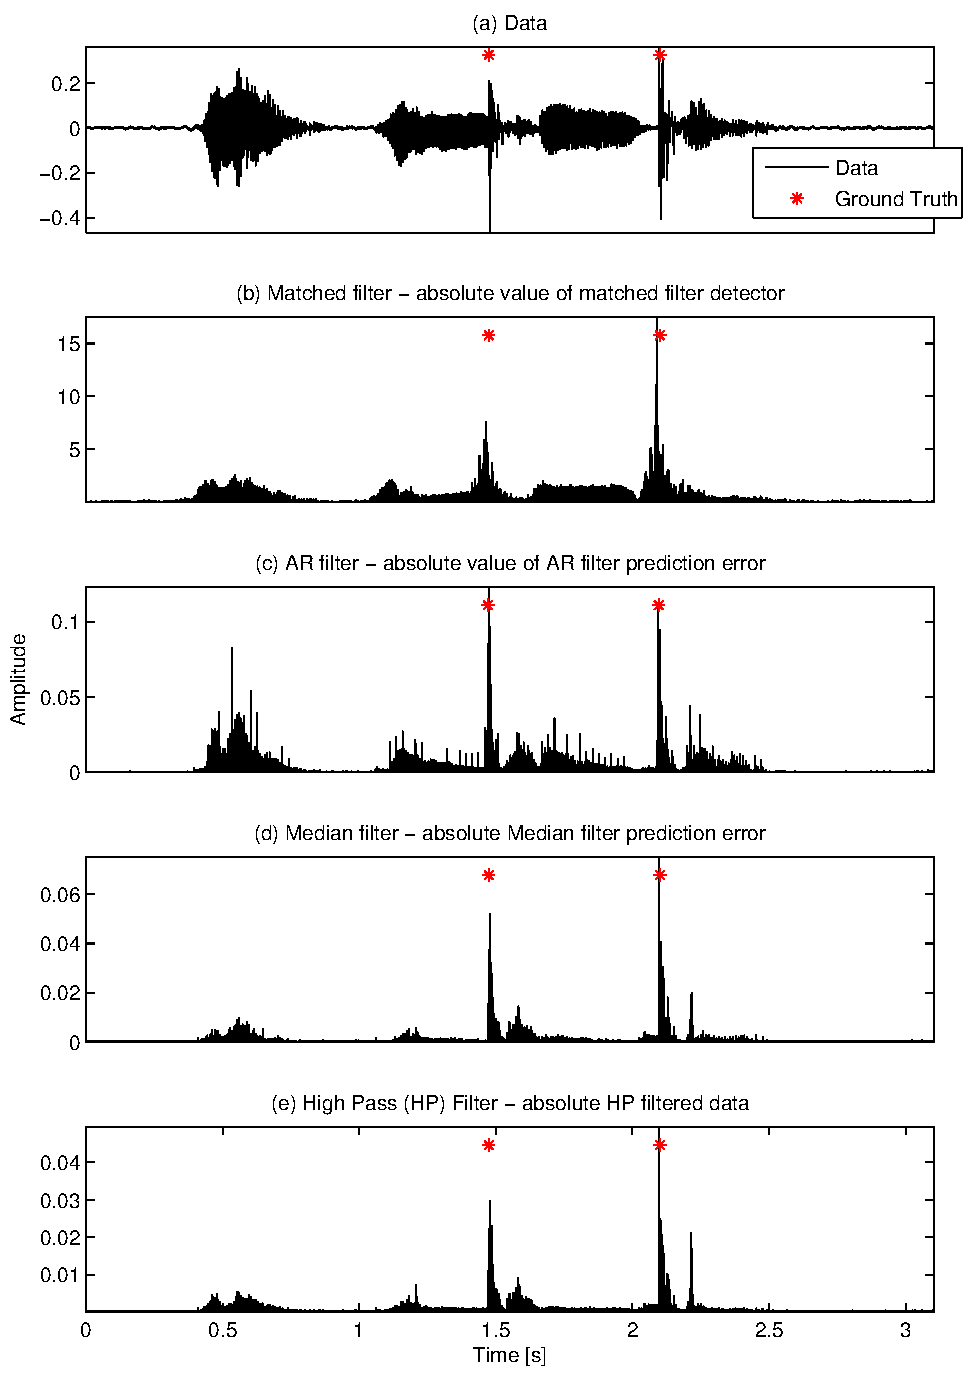
\includegraphics[width=130mm]{LitRev_DetectCompare2.pdf}
\caption{Impulse detection comparison, (a) Speech data with 2 primary keystroke impulses sampled at 44.1 kHz, (b) absolute value matched filter detector output, (c) absolute value of AR filter prediction error output, (d) absolute value of median filter prediction error, and (e) absolute value of high pass filtered data with crossover frequency 9.6 kHz.}
\label{fig:LitRev_DetectCompare2}
\end{figure}

%Warped linear prediction
Warped Linear Prediction (WLP) is another adaptation of the AR method \cite{Esquef2002}. The basic area of \emph{warped} DSP was first introduced in \cite{Oppenheim1983} and later formalized in a predictive framework in \cite{Strube1980} and as a recursive filter\cite{Steiglitz1980}. WLP has since been applied successfully to several audio applications \cite{Karjalainen1997}\cite{Haermae2000} and more specifically used as a basis for impulse detection \cite{Esquef2000}\cite{Esquef2002}.

The basic concept of warped filters can be explained by considering a standard FIR-like structure, but rather than applying the standard unit delay $z^{-1}$ the warped filter applies a new delay element $D(z)$ so that each new delay is frequency dependant (dispersive). In practice this means that the design of the warped filters are based on any pair of functions, $\tilde{z} = f(z)$ and $z = g(\tilde{z})$, so that $f(\cdot)$ and $g(\cdot)$ are one-to-one mappings of the unit circle onto itself, and $z = g\left( f(z) \right)$\cite{Karjalainen1997}. Bilinear conformal mapping\cite{Brown1996} conforms to the requirements and corresponds to the first order allpass filter

\begin{equation}\label{eq:Karjalainen1997}
\tilde{z}^{-1} = D(z) = \frac{z^{-1} - \lambda}{1 - \lambda z^{-1}},
\end{equation}

where $\lambda, -1 < \lambda < 1$, is a warping parameter which, if chosen appropriately \cite{Karjalainen1997}, yields a good match to the psychoacoustic Bark scale\cite{Smith1995}.

Warped digital filters have a range of advantages in that they can be designed to model the human auditory system as well as other physical systems\cite{Karjalainen1997}. In \cite{Esquef2002} the authors note that for auditory models the warping factor $\lambda$ tend to be positive while for click detection negative warping factors appeared to perform best. It was also noted that impulse detection using WLP came at a computational cost and was therefore not suited for real time implementations. As in \cite{Godsill1998book} the authors of \cite{Esquef2002} only considered impulses with duration of $<1 ms$, for which the WLP based method performs well. This is largely believed to be caused by spectral characteristics also exploited in \cite{Kasparis1993}\cite{US6795559}, although the signals in \cite{Esquef2002} were not exclusively corrupted speech data and can therefore not be assumed to be spectrally sparse at high frequencies.

\subsection{Frequency methods}
Others have attempted to use the STFT as a basis for detection \cite{Czyzewski1995}\cite{Subramanya2007}\cite{Sugiyama2007} causing problems such as loss of temporal resolution of detections at moderate frame sizes, loss of spectral resolution for smaller frame size and computational inefficiency using extensive overlapping of frames. The authors of \cite{Subramanya2007} propose an algorithm for detection of keystroke noise on laptop computers and recognise the temporal and spectral variability in the noise pulses causes methods based on noise models and stationarity assumptions to perform poorly. Instead the authors propose to exploit the ``smoothness in speech signals present across time'' and the relative spectral sparsity of speech signals compared to keystroke noise pulses with a simple linear predictive model across each frequency bin. Their model assumes that

\begin{equation}
\label{eq:Subramanya2007}
S(k,t) = \sum_{m=1}^M \alpha_{km} S(k,t - \tau_m) + V(k,t),
\end{equation}

where, $S(k,t)$ represents the time-frequency component for $k$ and $t$, spectral and time index respectively, $\boldsymbol{\tau} = \left\{\tau_1, \ldots ,\tau_M \right\}$ defines the frames used, $\boldsymbol{\alpha}_k = \left\{\alpha_{k1},\ldots,\alpha_{kM} \right\}$ define the weights used for the linear prediction, and $V(t,k)$ is some zero-mean Gaussian noise with variance $\sigma^2_{tk}$.

The authors of \cite{Subramanya2007} proceed to calculate the joint probability assuming independent frequency frames and eventually the log-likelihood $F_t$ will be

\begin{equation}
\label{eq:Subramanya2007_2}
F_t = - \frac{1}{2} \sum_k \frac{1}{\sigma^2_{tk}} \left( S\left(k,t\right) - \sum_{m=1}^M \alpha_{km} S(k,t-\tau_m)\right)^2 + C_{tk}
\end{equation}

where $C_{tk}$ is a constant.

\subsubsection{Time-Frequency processing}
Since the object of interest in our detection efforts is inherently transient and therefore localised in time, it is a significant shortcoming of classic Fourier analysis that it provides no such temporal information. The basics of time-frequency processing is the correlation of a signal with a family of waveforms that are well concentrated in time as well as in frequency\cite{Mallat1999} also called \emph{time-frequency atoms}\cite{Gabor1946}. The popular STFT used in numerous applications dates back to 1946 and the introduction of the windowed Fourier atoms to measure the ``frequency variations'' of sound. Given the real and symmetric window

\begin{equation}\label{eq:Mallat1999}
g_{u,\xi}(t) = \mathrm{e}^{i\xi t}g(t-u),
\end{equation}
where $\xi$ is a modulation frequency and $u$ is a translation and normalized $\|g\| = 1$ so that $\|g_{u,\xi}\| = 1$ for any $(u, \xi) \in \mathbb{R}^2$. The resulting windowed Fourier transform of $f \in \mathbf{L^2}(\mathbb{R})$ is

\begin{equation}\label{eq:Mallat1999_2}
S f(u, \xi) = \langle f, g_{u,\xi} \rangle = \int^{+\infty}_{-\infty}  f(t)g(t-u)\mathrm{e}^{-i\xi t} dt,
\end{equation}
which is also called the Short Time Fourier Transform (STFT) since the window $g(t-u)$ has the effect of localising the Fourier integral in the region of $t=u$.

To evaluate the energy density $P_S$ of the STFT, also called the \emph{spectrogram}, the squared magnitude is computed:

\begin{equation}\label{eq:Mallat1999_3}
P_S f(u,\xi) = |S f(u,\xi)|^2 = \left| \int^{+\infty}_{-\infty} f(t)g(t-u)\mathrm{e}^{-i\xi t} dt \right|^2.
\end{equation}

The \emph{spectrogram} of $f$ is a measure of the energy in the time-frequency neighborhood of $(u,\xi)$. This is also called the Heisenberg box of $g_{u,\xi}$ and is defined as a region in the time-frequency plane $(t, \omega)$ whose location and width depends entirely on the time-frequency spread of the window $g_{u,\xi}$ centered around $(u,\xi)$\cite{Mallat1999}.

For the windowed Fourier transform the time spread $\sigma_t$ and frequency spread $\sigma_w$ are independent of $u$ and $\xi$. \todo{Add appendix of 4.12-4.15 Mallat1999}Therefore $g_{u,\xi}$ corresponds to a Heisenberg box of area $\sigma_t \sigma_\omega$ centered at $(u,\xi)$ as seen in Figure~\ref{fig:LitRev_HeisenbergBox_STFT}\cite{Heisenberg1927}. The size of the box is constant and therefore independent of $(u,\xi)$ meaning that the windowed Fourier transform has the same temporal and frequency resolution throughout the time-frequency plane\cite{Mallat1999}.

\begin{figure}[!] %LitRev_HeisenbergBox_STFT
\centering
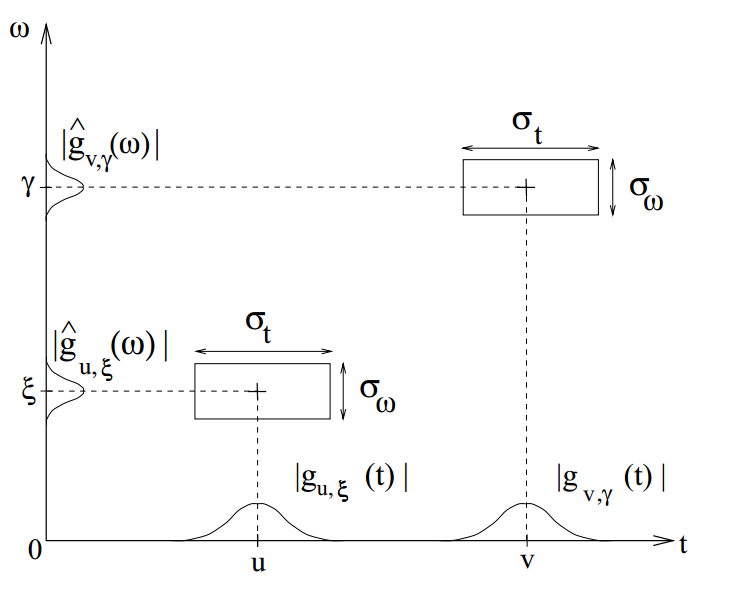
\includegraphics[width=80mm]{LitRev_HeisenbergBox_STFT.png}
\begin{picture}(0,0)
%\put(-355,120){Frequency}
%\put(-200,0){Time}
\end{picture}
\caption{An example of the Heisenberg box illustration and the inherent time-frequency resolution trade-off for the STFT.}
\label{fig:LitRev_HeisenbergBox_STFT}
\end{figure}

In practice this gives rise to a trade-off between temporal and frequency resolution, illustrated in Figure~\ref{fig:LitRev_STFTlims}, where two different temporal frame sizes are shown in relation to the resulting frequency resolution.

\subsubsection{Wavelet decomposition}
The Wavelet Transform can be seen as a generalization of the windowed Fourier transform in that it decomposes a signal over dilated and translated wavelets. A wavelet is simply a function $\phi \in \mathbf{L^2}(\mathbb{R})$ which is normalised $\| \phi \| = 1$, centered in the neighborhood of $t=0$, and with zero average:

\begin{equation}\label{eq:Mallat1999_4}
\int^{+\infty}_{-\infty} \psi(t) dt = 0.
\end{equation}

Unlike the windowed Fourier transform the family of time-frequency wavelet atoms is translated by $u$ as well as scaled by $s$:

\begin{equation}\label{eq:Mallat1999_5}
\phi_{i,s}(t) = \frac{1}{\sqrt{s}}\psi\left(\frac{t-u}{s}\right).
\end{equation}

Now we have that the wavelet transform of $f \in \mathbf{L^2}(\mathbb{R})$ at time $u$ and scale $s$ is

\begin{equation}\label{eq:Mallat1999_x}
W f(u,s) = \langle f, \psi_{u,s} \rangle = \int^{+infty}_{-\infty} = f(t) \frac{1}{\sqrt{s}}\psi^\ast \left( \frac{t-u}{s} \right) dt.
\end{equation}

%continue on reasoning from eq 4.50 Mallat 1999
\todo{Add appendix of 4.50-4.55 Mallat1999}

The energy spread of a wavelet time-frequency atom $\phi_{u,s}$ corresponds to a Heisenberg box centered at $(u,\eta/s)$ where $\eta$ is the center frequency of $\hat{\phi}$ the Fourier transform of $\phi$, and $\hat{\phi_{u,s}}$ is the Fourier transform of $\phi$ dilated by $1/s$ \todo{refer to appendix}. The Heisenberg box remains of area $\sigma_t \sigma_\omega$ at all scales but it is now $s\sigma_t$ on the time axis and $\sigma_\omega /s$ along the frequency axis. The temporal and frequency resolution is now dependent on $s$ as illustrated in Figure~\ref{fig:LitRev_HeisenbergBox_wavelets}

\begin{figure}[!] %LitRev_HeisenbergBox_wavelets
\centering
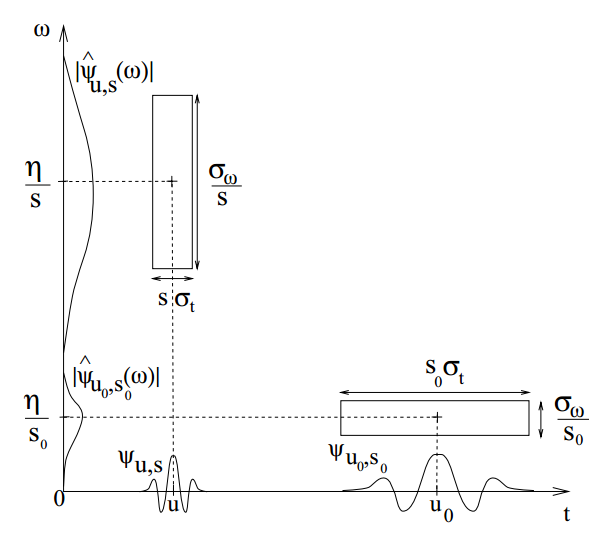
\includegraphics[width=80mm]{LitRev_HeisenbergBox_wavelets.png}
\begin{picture}(0,0)
%\put(-355,120){Frequency}
%\put(-200,0){Time}
\end{picture}
\caption{The Heisenberg boxes for the wavelet transform.}
\label{fig:LitRev_HeisenbergBox_wavelets}
\end{figure}

The main difference between classic Fourier analysis and Wavelet analysis is that Wavelets are localised in both frequency and time whereas the Fourier transform is only localised in frequency. This leads to some significant advantages when considering data that is inherently transient. While the Short Time Fourier Transform (STFT) does, to an extent, mimic the time localisation of the Wavelet Transform it does so at the cost of temporal resolution\cite{Mallat1999}. This inherent trade-off between temporal and frequency resolution is illustrated in Figure~\ref{fig:LitRev_STFTlims} where two different temporal frame sizes are shown in relation to the resulting frequency resolution.

%LitRev_STFTlims
\begin{figure}
\centering
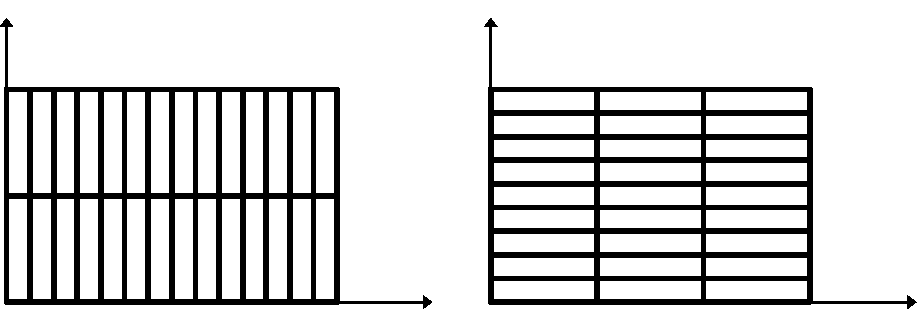
\includegraphics[width=120mm]{LitRev_STFTlims.pdf}
\begin{picture}(0,0)
\put(-355,120){Frequency}
\put(-200,0){Time}
\put(-175,120){Frequency}
\put(-20,00){Time}
\end{picture}
\caption{Heisenberg boxes of two wavelets. At larger scales the frequency resolution is increased by a decreased frequency support and the time spread is increased.}
\label{fig:LitRev_STFTlims}
\end{figure}

%LitRev_Wavelets
\begin{figure}
\centering
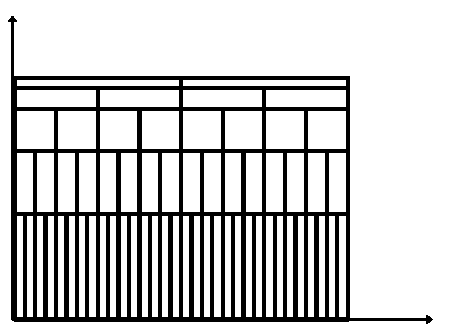
\includegraphics[width=65mm]{LitRev_Wavelets.pdf}
\begin{picture}(0,0)
\put(-195,133){Scale}
\put(-22,-7){Time}
\end{picture}
\caption{The scale-time relationship for the wavelet transform.}
\label{fig:LitRev_Wavelets}
\end{figure}

Figure~\ref{fig:LitRev_Wavelets} shows a similar plot to Figure~\ref{fig:LitRev_STFTlims} but for the Wavelet transform instead. It should be noted that a Wavelet spectrum, equivalent to a traditional spectrogram, is traditionally plotted in the time-scale space, where scale can be seen as being inversely proportional to frequency.

\subsubsection{Multi-resolution analysis with Filter Banks}
Consider now the discrete power spectral density calculation, from Equation~\ref{eq:Mallat1999_3}, for the signal $x(n)$:
%Add description for filter bank paradigm here

\begin{equation}\label{eq:LitRev_Detection_PSD1}
S_{xx}(\omega) = \frac{1}{N} \left| \sum^{N}_{n=1} x(n) e^{-i \omega n} \right|^2.
\end{equation}

For a given frequency $\omega_i$, equation~\ref{eq:LitRev_Detection_PSD1} can be rewritten as

\begin{equation}\label{eq:LitRev_Detection_PSD2}
S_{xx}(\omega_i) = \left\| \sum^{N}_{k=1} h_i(k) x(n-k) \right\|^2,
\end{equation}

where

\begin{equation}\label{eq:LitRev_Detection_PSD3}
h_i(k) = w(k)e^{-i \omega_i n},
\end{equation}

and $w(k)$ is a window function. Considering $w(k)$ as a prototypical FIR lowpass filter, the collection of all $h_i(k)$s constitutes a bank of bandpass filters each centered on frequency $\omega_i$\cite{Ariananda2013}. This implementation is commonly referred to as the periodogram but it also highlights what sometimes is called the filter bank paradigm and is a particularly simple implementation of the DWT\cite{Mallat1999}.

Considering again the window function $w(k)$ from equation~\ref{eq:LitRev_Detection_PSD3}, the simplest window conceivable would be a simple rectangular window $w(k) = 1/N$. Naturally this would lead to significant side lobe leaks in the spectral domain and is therefore highly undesirable. Employing Hamming and Hann windows is a common approach to alleviate these issues. Another issue that arises with the periodogram is that its estimates are coarse with low precision and large variance\cite{Ariananda2013}. A common method for alleviating this variance problem is by windowing the data first\cite{Lim1988book}.

Work done on Multi Taper Spectrum Estimation (MTSE)\cite{Thomson1982} and later on multi-resolution theory\cite{Mallat1989}\cite{Meyer1995} proves that conjugate mirror filter characterizes a wavelet and that cascading these filters will lead to a fast implementation of the discrete wavelet transform.

Figure~\ref{fig:LitRev_DWTstep.pdf} shows a diagrammatic representation of a single step of the DWT. The \emph{Lo} and \emph{Hi-pass} filters represent, respectively, the low and high pass conjugate mirror filters and the following step is a dyadic decimation (down-sampling) step. Since the spectrum of each filtered signal is effectively halved by the filters, the decimation step removes redundant information in accordance with Nyquist's theorem. The output of the low and high-pass filters are commonly referred to as the approximation and the detail coefficients respectively\cite{Mallat1999}.

%LitRev_DWTstep.pdf
\begin{figure}
\centering
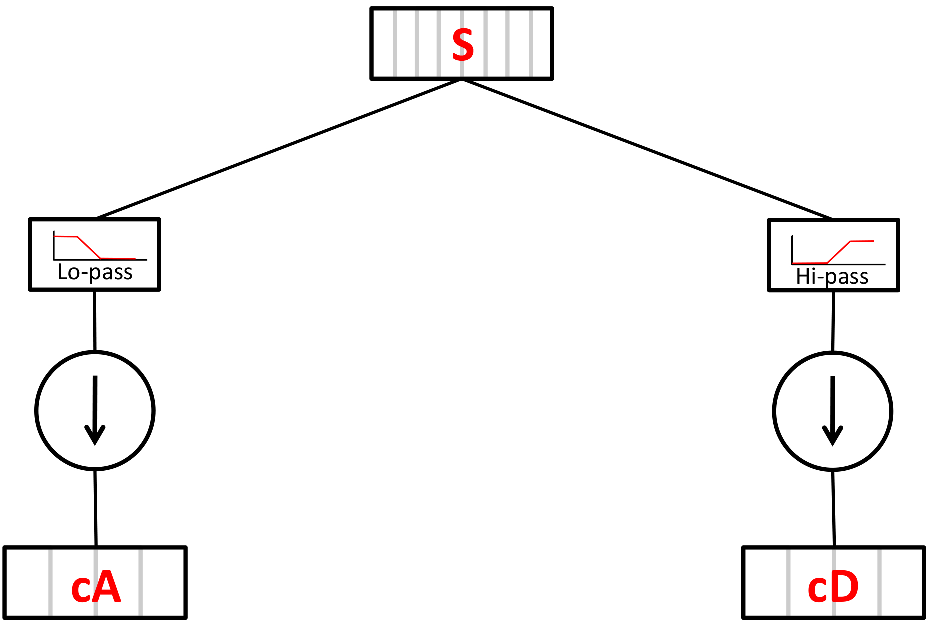
\includegraphics[width=85mm]{LitRev_DWTstep.pdf}
\begin{picture}(0,0)
%\put(-195,133){Scale}
%\put(-22,-7){Time}
\end{picture}
\caption{A single wavelet decomposition step.}
\label{fig:LitRev_DWTstep.pdf}
\end{figure}

Figure~\ref{fig:LitRev_DWTtree.pdf} shows a three level wavelet decomposition. 
%LitRev_DWTtree.pdf
\begin{figure}
\centering
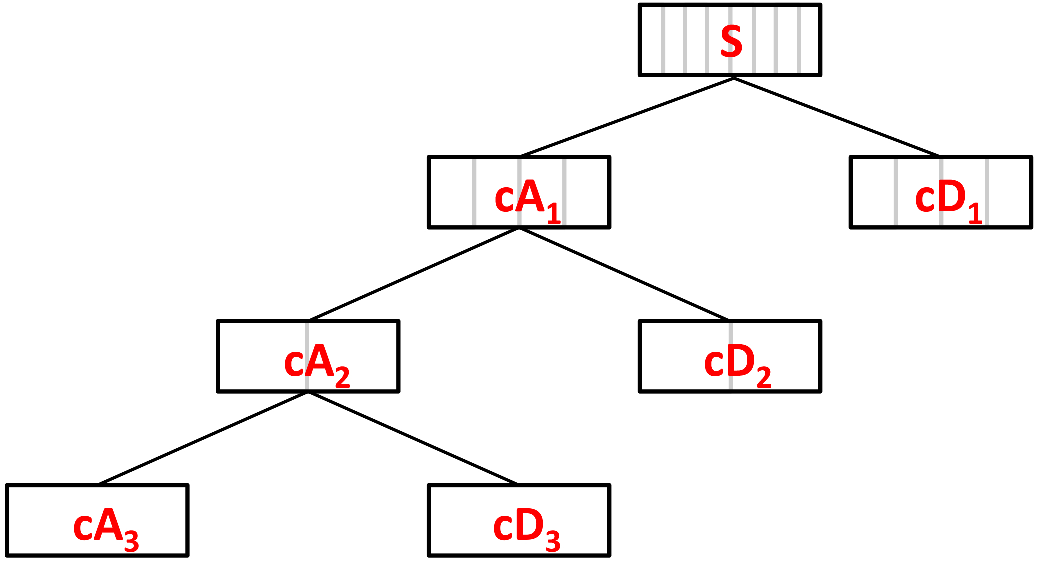
\includegraphics[width=85mm]{LitRev_DWTtree.pdf}
\begin{picture}(0,0)
%\put(-195,133){Scale}
%\put(-22,-7){Time}
\end{picture}
\caption{Three level wavelet decomposition tree.}
\label{fig:LitRev_DWTtree.pdf}
\end{figure}


The multi-resolution properties of the wavelet transform has made the Wavelet transform popular in a range of audio and speech applications where much of the information of interest is located in the lower frequency bands\cite{Sinha1993}\cite{Czyzewski1995}\cite{Lambrou1998}\cite{Tzanetakis2001}\cite{Zurera2001}\cite{Lin2005}. Equally the computational efficiency of the discrete wavelet transform is cited\cite{Kadambe1992} as a significant advantage over the FFT with an $O(N)$ complexity compared to $O(N\mathrm{log}(N)$ for FFT\cite{Mallat1999}. In \cite{Kadambe1992} the authors report ``superior pitch detection performance'' citing the Wavelet transforms computational efficiency, temporal resolution and its suitability of the pitch periods found in the analysed material. Speech applications in particular report good spectral estimation capabilities \cite{Hu2004}, good de-noising capabilities \cite{Donoho1995}\cite{Seok1997}, and good compression performance \cite{Sinha1993}\cite{Fgee1999}. Several authors propose wavelets used as a bases for audio classification applications\cite{Lambrou1998}\cite{Tzanetakis2001}\cite{Lin2005} and report that a specific advantage of the wavelet basis is its compact representation compared to the time domain signal which decreases processing delay/cost\cite{Lambrou1998}.

An early wavelet based click detection algorithm proposes to detect clicks by analysing the wavelet coefficients of the signal for discontinuities\cite{Czyzewski1995}. The authors apply a neural network algorithm to robustly detect and classify impulses although the authors note that the required training stage is both ``a complex and time-consuming procedure''. While not explicitly discussed the authors appear to be targeting extremely short time impulses of the order of 1 or 2 samples, or what they call ``parazite impulses''.


\subsubsection{Wavelet Packet Transform (WPT)}
\todo{Wavelet Packet Transform review}
%introduced by: \cite{Coifman1992a}
The Wavelet Packet Transform (WPT) can be seen as a generalisation of the Wavelet transform in that it extends the link between multi-resolution approximations and wavelets. The WPT can also be seen as a natural extension of MSTE\cite{Thomson1982}. While the DWT decomposes only the approximation coefficients the WPT applies the decomposition step symmetrically throughout the tree as seen in Figure~\ref{fig:LitRev_WPTtree.pdf}. Since the standard DWT algorithm is limited to wavelet bases that increase by a power of two towards the higher scales (low frequencies) it is possible that some other combination of bases could provide a better basis in some applications\cite{Coifman1992a}.


%LitRev_WPTtree.pdf
\begin{figure}
\centering
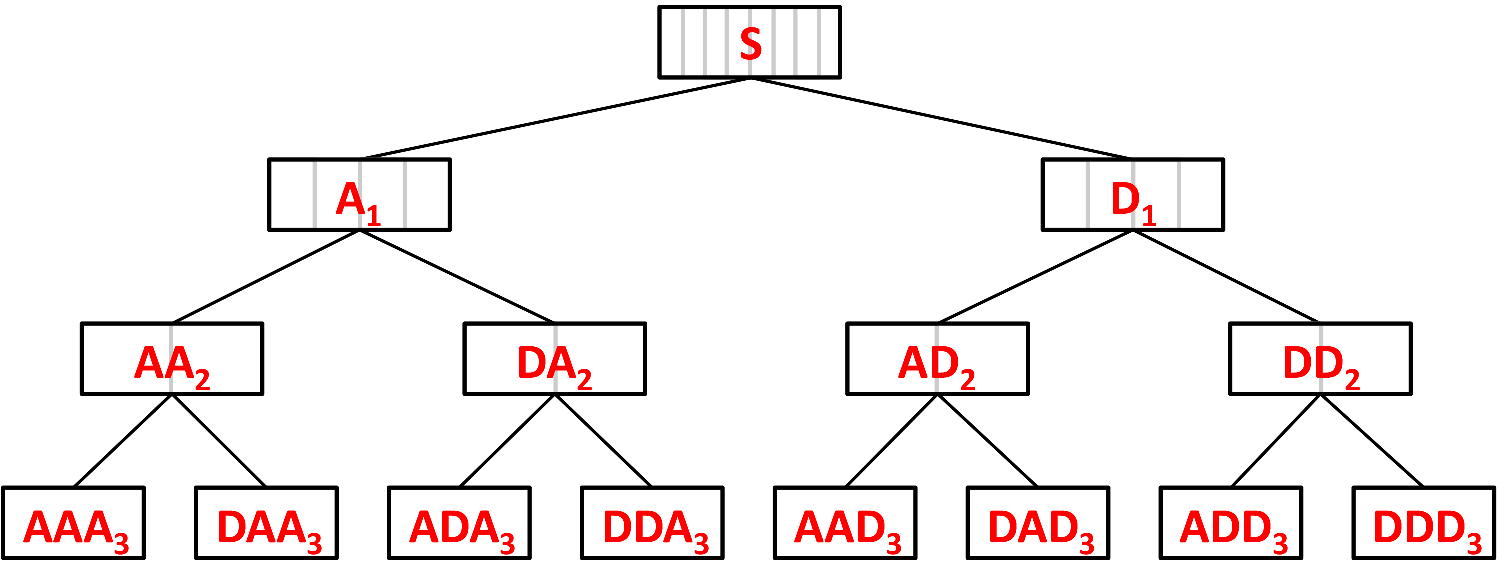
\includegraphics[width=125mm]{LitRev_WPTtree.pdf}
\begin{picture}(0,0)
%\put(-195,133){Scale}
%\put(-22,-7){Time}
\end{picture}
\caption{Three level wavelet packet decomposition tree.}
\label{fig:LitRev_WPTtree.pdf}
\end{figure}

In a recent study comparing the WPT to other spectrum estimation techniques it was generally found that the WPT ``operated well for all types of sources and its performances were comparable or at times even better than other existing approaches.''\cite{Ariananda2013}. In particular it was found that WPT performed well in reducing variance in the stop bands.

The authors of \cite{He2008} developed a psychoacoustic model based around the WPT and found that not only was the WPT computationally more efficient than a Fourier transform-based alternative but it also provided a better spectral resolution. For psychoacoustic applications it was found that the generalization of the DWT yielded a better approximation of the critical bands employed\cite{Carnero1999}\cite{He2008} compared to similar DWT based models\cite{Sinha1993}\cite{Zurera2001}.

\todo{Needs rewriting. ->}
Due to the compactly supported nature of the wavelet\cite{Mallat1999} these shortcomings can be mitigated \cite{Nongpiur2008} and provide a useful basis for the removal of impulses with little to no noticeable degradation of the signal. Further, direct statistical modeling the noise pulses and background signals allows for probabilistic inference \cite{Godsill1998} with potentially very high accuracy, and in this case greatly simplifies calculations and implementation.
\todo{<-}

\section{Restoration}\label{sec:LitRev_Restoration}
The restoration of corrupted speech and audio samples by a localised degradation, also referred to as clicks or noise pulses, has inspired much research and many approaches. Corruptions can generally be seen to have varying severity. Short clicks have traditionally been treated as completely corrupted or essentially missing transforming the restoration task into one of interpolation of missing samples\cite{Godsill1998book}\cite{Tukey1977}\cite{Tukey1974}.

%literature review
%\cite{Vaseghi1990}: LSE estimates with LPC model. Long term correlation structure

%\cite{Windyga2001}, \cite{Alajlan2004}: Non-linear, minimum or maximum of neighborhood based on dark or bright spot. (Alajlan based on Windyga, good explanation of Windyga in Alajlan)

%\cite{Czyzewski1995}: LPC and maybe more (meta analysis)

%Median filtering for restoration:
%JAYNAT, N.S.: ‘Average and median based smoothing for improving
%digital speech quality in the presence of transmission errors’,
%IEEE Trans., COM-24,1976, pp. 1043-1045
%
% ^ Efficacy of employing some simple waveform smoothing. Transmission errors.
%
%KUNDA, A.: ‘Applications of a two dimensional generalised mean
%filtering for removal of impulsive noise from images’, IEEE 7rans.,
%ASP-23, (6), 1984, pp. 552-557
%Weighted mean, black and white photos, very simple!
%
%RABINER, L.R., SAMBUR, M.R., and SCHMIDT, C.Es
%of a nonlinear smoothing algorithm to speech processing.
%IEEE Trans., ASSP-32, (3), 1984‘
%
% ^ Median and linear smoothing combined.
%   Linear smoothing is rarely enough.
%
% "Generalized median filtering and related nonlinear filtering techniques"
% Another median+linear smoother

%Median LPC hybrid
%NIEMINEN, HEINONEN, P., and NEUVO, Y.: ‘Suppression
%and detection of impulsive type interference using adaptive median
%hybrid filter’. IEEE Proc. ICASSP 1987, pp. 117-120.

% AR \cite{Janssen1986}

%\subsection{Median filtering}



%\section{Residual Restoration}
A variety of restoration algorithms have been tested for the restoration of the residual audio component. Based on the nature of the detection algorithm, the restoration step can be done either on the wavelet coefficients or on the time series data.

\todo{something more}





% ------------------------------------------------------------------------


%%% Local Variables:
%%% mode: latex
%%% TeX-master: "../thesis"
%%% End:



